\documentclass[tikz,border=10pt]{standalone}
\usepackage{tikz}
\usetikzlibrary{shapes.geometric, arrows, positioning}

\begin{document}

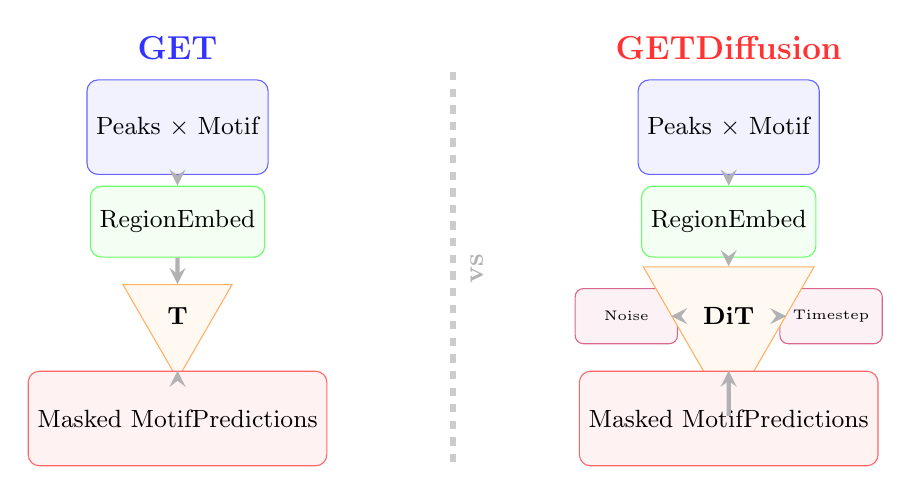
\begin{tikzpicture}[
    % Node styles
    input/.style={rectangle, draw=blue!60, fill=blue!5, rounded corners=4pt, 
                  minimum width=2.2cm, minimum height=1.2cm, text centered, font=\small},
    embed/.style={rectangle, draw=green!60, fill=green!5, rounded corners=4pt,
                  minimum width=2.2cm, minimum height=0.9cm, text centered, font=\small},
    encoder/.style={regular polygon, regular polygon sides=3, draw=orange!60, 
                    fill=orange!5, minimum size=1.6cm, text centered, font=\small\bfseries,
                    shape border rotate=180},
    output/.style={rectangle, draw=red!60, fill=red!5, rounded corners=4pt,
                   minimum width=2.2cm, minimum height=1.2cm, text centered, font=\small},
    noise/.style={rectangle, draw=purple!60, fill=purple!5, rounded corners=3pt,
                  minimum width=1.3cm, minimum height=0.7cm, text centered, font=\tiny},
    arrow/.style={->, >=stealth, line width=1.5pt, color=gray!60}
]

% Left side: GETRegionPretrain
\begin{scope}[xshift=0cm]
    % Title
    \node[font=\large\bfseries, yshift=3.8cm, color=blue!80] at (0,0) {GET};
    
    % Input
    \node[input] (input1) at (0,2.8) {Peaks $\times$ Motif};
    
    % Embedding
    \node[embed] (embed1) at (0,1.6) {RegionEmbed};
    
    % Encoder
    \node[encoder] (encoder1) at (0,0.4) {T};
    \node[font=\tiny, below=0.15cm of encoder1, color=gray!70] {Transformer};
    
    % Output
    \node[output] (output1) at (0,-0.9) {Masked Motif\\Predictions};
    
    % Arrows
    \draw[arrow] (input1) -- (embed1);
    \draw[arrow] (embed1) -- (encoder1);
    \draw[arrow] (encoder1) -- (output1);
\end{scope}

% Right side: GETRegionDiffusion
\begin{scope}[xshift=7cm]
    % Title
    \node[font=\large\bfseries, yshift=3.8cm, color=red!80] at (0,0) {GETDiffusion};
    
    % Input
    \node[input] (input2) at (0,2.8) {Peaks $\times$ Motif};
    
    % Embedding
    \node[embed] (embed2) at (0,1.6) {RegionEmbed};
    
    % Noise and Timestep (positioned to sides of encoder)
    \node[noise] (noise) at (-1.3,0.4) {Noise};
    \node[noise] (timestep) at (1.3,0.4) {Timestep};
    
    % Encoder
    \node[encoder] (encoder2) at (0,0.4) {DiT};
    \node[font=\tiny, below=0.15cm of encoder2, color=gray!70] {DiT Encoder};
    
    % Output
    \node[output] (output2) at (0,-0.9) {Masked Motif\\Predictions};
    
    % Arrows
    \draw[arrow] (input2) -- (embed2);
    \draw[arrow] (embed2) -- (encoder2);
    \draw[arrow] (noise) -- (encoder2);
    \draw[arrow] (timestep) -- (encoder2);
    \draw[arrow] (encoder2) -- (output2);
\end{scope}

% Comparison separator
\draw[line width=2pt, dashed, color=gray!40] (3.5,3.5) -- (3.5,-1.5);
\node[font=\normalsize\bfseries, color=gray!60, rotate=90] at (3.8,1) {vs};

\end{tikzpicture}

\end{document}

